\documentclass[a4paper, 12pt, oneside]{report}

\usepackage[a4paper, left=3.5cm, right=2.5cm, bottom=2.5cm, top=2.5cm]{geometry}

% polskie znaki
\usepackage[OT4,plmath]{polski}
\usepackage[utf8]{inputenc}

\usepackage[T1]{fontenc}
\usepackage{graphicx}
\usepackage{epsfig}
\usepackage{epstopdf}
\usepackage[usenames,dvipsnames]{color}
\usepackage{url}
\usepackage{indentfirst}
\usepackage{hyperref}
\usepackage{listings}
\usepackage{caption}
\usepackage{textcomp}
\usepackage{amsmath}
\usepackage{needspace}
\usepackage{etoolbox}
\usepackage{longtable}
\usepackage{lipsum}
\usepackage{multirow}
\usepackage{amsfonts}
\usepackage{strona_tytulowa}

\graphicspath{{rys/}}

\lstset{
    inputpath=../connect4,
    frame=top,
    numbers=none,
    stepnumber=1,
    numbersep=10pt,
    tabsize=4,
    extendedchars=true,
    breaklines=true,
    captionpos=t,
    %mathescape=true,
    showspaces=false,
    showtabs=false,
    xleftmargin=0pt,
    framexleftmargin=0pt,
    framexbottommargin=0pt,
    framextopmargin=5pt,
    showstringspaces=false,
    upquote=true,
    belowskip=1em
}

\lstdefinestyle{numbers}{
    numbers=left
}

\lstset{literate={ą}{{\k{a}}}1 {ł}{{\l{}}}1 {ń}{{\'n}}1 {ę}{{\k{e}}}1 {ś}{{\'s}}1 {ż}{{\.z}}1 {ó}{{\'o}}1 {ź}{{\'z}}1 {Ą}{{\k{A}}}1 {Ł}{{\L{}}}1 {Ń}{{\'N}}1 {Ę}{{\k{E}}}1 {Ś}{{\'S}}1 {Ż}{{\.Z}}1 {Ó}{{\'O}}1 {Ź}{{\'Z}}1 }

\makeatletter
\patchcmd{\lst@GLI@}% <command>
  {\def\lst@firstline{#1\relax}}% <search>
  {\def\lst@firstline{#1\relax}\def\lst@firstnumber{#1\relax}}% <replace>
  {\typeout{listings firstnumber=firstline}}% <success>
  {\typeout{listings firstnumber not set}}% <failure>
\makeatother

\DeclareCaptionFormat{listing}{\textbf{#1#2}#3}
\captionsetup[lstlisting]{format=listing,singlelinecheck=false, margin=0pt, font={sf},labelsep=space,labelfont=bf}

\renewcommand\lstlistingname{Listing}

\title{\MakeUppercase{Zastosowanie uczenia ze wzmocnieniem w~doborze strategii reprezentowanej przez sieć neuronową w~grze planszowej Connect~4}}
\author{Jakub Młokosiewicz}
\album{26875}
\kierunek{Informatyka}
\specjalnosc{Systemy komputerowe i~oprogramowanie}
\forma{stacjonarne}
\angtitle{\MakeUppercase{Application of the reinforcement learning in~searching of the policy 
represented by~the~neural network for Connect 4} \\ \MakeUppercase{board game}}
\praca{inżynierska}
\promotor{dr inż. Marcina Plucińskiego}
\katedra{Katedra Metod Sztucznej Inteligencji i~Matematyki Stosowanej}
\datatematu{21.11.2014}
\datazlozenia{29.04.2016}
\rok{2016}

\begin{document}

\thispagestyle{empty}
{\sffamily \stronatytulowa }

\begin{titlepage}

\begin{center}
\vspace{2.cm}                   
\LARGE Application of the reinforcement learning in searching of the policy 
represented by the neural network for Connect 4 board game \\ 
\vspace{1cm}
\large Jakub Młokosiewicz\\
\large Supervisor: dr inż. Marcin Pluciński\\
\vspace{1cm}
\end{center}

\textbf{Abstract}
\vspace{12pt}

There are two basic ways of solving the problem of playing board games alghoritmically -- searching the game tree, and learning by interaction with the environment. In the first case it is necessary to define a~method of board state evaluation. Reinforcement learning is an example of the latter approach involving agent learning to make good decisions based on received (delayed) reinforcements.

The main goal of the thesis is to design and implement an alghoritm based on reinforcement learning which would allow learning a~policy for Connect 4 board game granted that it is represented by an artificial neural network. The secondary objective is to develop application allowing the practical realisation of learning and testing its results.

\end{titlepage}

\pagebreak

{\sffamily % ------------------------------------------------------------------------
% Wzór pracy dyplomowej zgodnie ze wzorcem
% obowiązującym na Wydziale Informatyki ZUT
% data: 27.06.2011-07.02.2016
% autor: J. Kołodziejczyk
% 
% Preambuła: oświadczenie o samodzielnie wykonanej pracy
% ------------------------------------------------------------------------

\addcontentsline{toc}{chapter}{Oświadczenie }
\begin{center}
\textbf{\large OŚWIADCZENIE \\AUTORA PRACY DYPLOMOWEJ}
\end{center}

\noindent Oświadczam, że praca dyplomowa inżynierska pt.

\noindent \textbf{Zastosowanie uczenia ze wzmocnieniem w~doborze strategii reprezentowanej przez sieć neuronową w grze planszowej Connect~4}

\noindent napisana pod kierunkiem:

\noindent \textbf{dr inż. Marcina Plucińskiego}

\noindent jest w całości moi samodzielnym autorskim opracowaniem sporządzonym przy wykorzystaniu wykazanej w pracy literatury przedmiotu i materiałów źródłowych.
\vspace{.5cm }

\noindent Złożona w~dziekanacie Wydziału Informatyki treść mojej pracy dyplomowej w formie elektronicznej jest zgodna z treścią w formie pisemnej.

\vspace{1cm }
\noindent Oświadczam ponadto, że złożona w dziekanacie praca dyplomowa ani jej fragmenty nie były wcześniej przedmiotem procedur procesu dyplomowania związanych z uzyskaniem tytułu zawodowego w uczeniach wyższych.
\vspace{1cm }

\flushright {....................................\\ podpis dyplomanta}

\flushleft 
\vspace{1cm }
Szczecin, dn. 29.04.2016
}

\tableofcontents
\listoftables
\addcontentsline{toc}{chapter}{Spis tabel}
\listoffigures
\addcontentsline{toc}{chapter}{Spis rysunków}

\chapter{Wprowadzenie}
 
 W~nauce istnieją obecnie dwa zasadnicze podejścia do problemu "maszynowego" grania w~gry planszowe -- budowanie i~przeszukiwanie drzewa gry oraz uczenie poprzez interakcje ze środowiskiem. W~tym pierwszym przypadku konieczne jest zdefiniowanie funkcji oceny sytuacji na planszy. Przykładem drugiego podejścia jest uczenie ze wzmocnieniem, polegające na uczeniu się przez agenta podejmowania odpowiednich decyzji na podstawie otrzymywanych opóźnionych w~czasie wzmocnień.

\section{Cel pracy}
Podstawowym celem pracy jest zaprojektowanie i~implementacja algorytmu bazującego na uczeniu ze wzmocnieniem, umożliwiającego uczenie się strategii dla gry Connect~4, przy założeniu, że jest ona reprezentowana przez sztuczną sieć neuronową. Celem dodatkowym jest opracowanie aplikacji umożliwiającej praktyczną realizację uczenia oraz testowania jego wyników.

\section{Struktura pracy}

Tak sformułowanym celom pracy podporządkowano jej układ. Rozdział drugi pościęcono grze Connect 4, będącej przedmiotem uczenia się ze wzmocnieniem, do którego wprowadzenie zawarto w~trzecim rozdziale pracy. Czwarty rozdział stanowi wprowadzenie do tematyki sieci neuronowych, zastosowanych w~niniejszej pracy jako aproksymator funkcji w~algorytmie uczenia ze wzmocnieniem. Opis zaprojektowanych i~zaimplementowanych jako cel pracy algorytmów został zawarty w~rozdziale piątym. Rozdział szósty zawiera opis badań wpływu poszczególnych współczynników na skuteczność uczenia się, przeprowadzonych z~wykorzystaniem wcześniej opisanych narzędzi.

\chapter{Gra Connect 4}

Gra Connect 4, w~Polsce znana także jako Czwórki, jest grą dla dwóch graczy, toczącą się na pionowo ustawionej planszy o~7 kolumnach i~6 wierszach. Gracze naprzemiennie wrzucają od góry swoje żetony, które opadają na dół, zajmując najniższe wolne miejsce w~kolumnie. Celem gry jest ułożenie obok siebie -- pionowo, poziomo lub na skos -- czterech swoich żetonów, zanim uczyni to przeciwnik \cite{wiki:ConnectFour}.

\begin{figure}[htp]
\centering
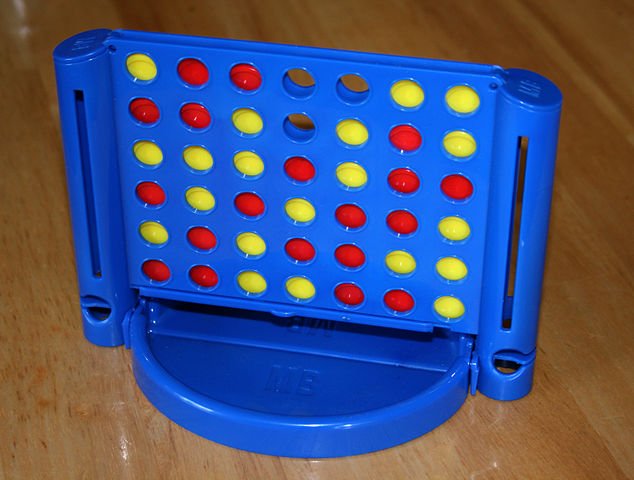
\includegraphics[scale=0.35]{connect4_plansza.jpg}
\caption{Przykładowa rozgrywka -- wygrał gracz grający czerwonymi żetonami\protect\footnotemark}
\label{fig:plansza}
\end{figure}
\footnotetext{Źródło: \url{https://commons.wikimedia.org/wiki/File:Connect_Four.jpg}}
 
Connect 4 jest grą o~pełnej informacji, co znaczy, że gracze grają naprzemiennie i~mają informację o~wszystkich ruchach, które miały miejsce, a~także o~wszyskich potencjalych ruchach, które można wykonać w~danym stanie gry. Connect 4 jest także grą o~sumie zerowej -- korzyść jednego gracza oznacza stratę drugiego \cite{wiki:ConnectFour}.

 W~klasycznym Connect 4 istnieje 4.531.985.219.092 \cite{EdelkampKissmann} pozycji możliwych do wystąpienia podczas gry. Warto jednak zauważyć, że większość z~tych stanów planszy występuje stosunkowo rzadko w~porównaniu do innych, częstszych oraz że większość pozycji posiada do pary stan odbity symetrycznie względem środkowej kolumny, równoważny względem planowania strategii gry.

\chapter{Uczenie ze wzmocnieniem}

Uczenie ze wzmocieniem ma za zadanie zamodelować problem uczenia się na podstawie interakcji z~otoczeniem, by ostatecznie osiągnąć zadany cel. Uczeń (zarazem jednostka podejmująca decyzje) nazywany jest \emph{agentem}. Wszystko poza nim nazywane jest \emph{środowiskiem}. Agent w~ciągły sposób wchodzi w~interakcje ze środowiskiem poprzez podejmowanie \emph{akcji}. W~odpowiedzi na nie, środowisko przedstawia agentowi swój nowy \emph{stan}. Środowisko daje agentowi \emph{wzmocnienia} o~wartościach dodatnich lub ujemnych. Agent stara się maksymalizować ich sumę \cite{SuttonBarto98}.

\begin{figure}[htp]
\centering
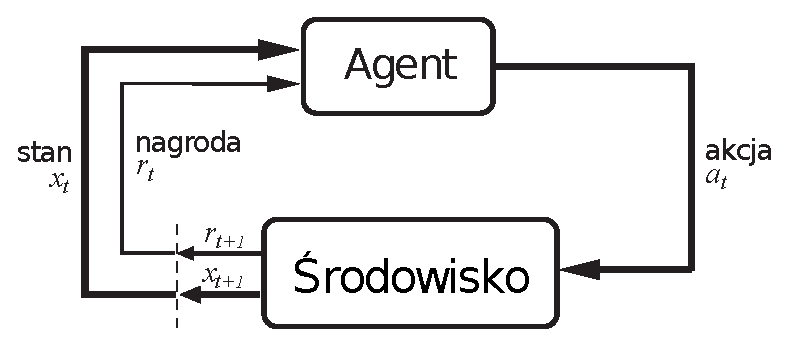
\includegraphics[scale=1.00]{rys/Agent-Env-pl.eps}
\caption{Interakcja agenta ze środowiskiem\protect\footnotemark}
\label{}
\end{figure}
\footnotetext{Diagram zaczerpnięty z~\cite{SuttonBarto98}. Tłumaczenie wykonane przez autora pracy.}

Agent oraz środowisko oddziałują na siebie w~dyskretnych krokach czasu, $t = 0, 1, 2, 3, ...$\footnote{Autorzy \cite{SuttonBarto98} wspominają w~tym miejscu, że czas można traktować również jako wartość ciągłą. Wybiega to jednak poza zakres niniejszej pracy.}. W~każdym kroku czasu $t$, agent obserwuje reprezentację stanu i~na jego podstawie wybiera akcję (należącą do zbioru akcji dostępnych w~tym stanie). W~kolejnym punkcie czasu, jako konsekwencję wybranej akcji, agent otrzymuje numeryczną nagrodę $r_t$ oraz przechodzi do nowego stanu \cite{SuttonBarto98}.

\section{Zadanie ucznia}

Jeśli zadanie do wykonania przez agenta przedstawione jest tylko w~postaci nagród, w~najbardziej ogólnym przypadku można powiedzieć, że tak naprawdę polega ono na nauczeniu się strategii, która będzie prowadziła do maksymalizacji sumy otrzymywanych nagród (i pośrednio do zdefiniowanego kryterium jakości, np. wygrania gry) \cite{Cichosz00}. Jednym z~przypadków jest ten, w~którym uczeń ma maksymalizować długoterminową sumę nagród -- w~tym ujęciu dobra strategia może okazać się opłacalna dopiero w~dłuższym horyzoncie czasowym. Biorąc pod uwagę ten typ uczenia można zdefiniować kryterium jakości, które system uczący powinien maksymalizować, w~postaci oczekiwanej zdyskontowanej sumy otrzymanych nagród:
\begin{equation}
\mathbb{E}\left[\sum_{t=0}^\infty\gamma^t r_t\right].
\end{equation}

Współczynnik dyskontowania $\gamma \in {[0, 1]}$ reguluje ważność krótko- i~długoterminowych nagród. Im większa wartość tego współczynnika, tym większe znaczenie mają przyszłe nagrody. W~szczególnym przypadku, gdy $\gamma=0$, uczeń będzie maksymalizował tylko natychmiastowe nagrody; natomiast gry $\gamma=1$, wzmocnienia ze wszystkich kroków czasu będą dla ucznia równie ważne i~brane pod uwagę.

Wiele praktycznych zadań ma charakter epizodyczny, to znaczy taki, że występuje \emph{stan absorbujący} kończący próbę. Równanie zdyskontowanej sumy otrzymanych nagród można wówczas sprowadzić do skończonego przypadku:
\begin{equation}
\mathbb{E}\left[\sum_{t=0}^{n-1}\gamma^t r_t\right],
\end{equation}
gdzie $n$ oznacza liczbę kroków próby.

 W~uczeniu się ze wzmocnieniem mamy do czynienia z~dwoma szczególnymi typami zadań strojących przed agentem. Cichosz nazywa je zadaniami do-sukcesu i~do-porażki \cite{Cichosz00}.

\subsubsection{Zadania do-sukcesu}
 W~zadaniach tego typu uczeń w~każdej kolejnej próbie ma za zadanie osiągnięcie pewnego celu, np. konkretnego stanu środowiska. Osiągniecie tego celu oznacza zakończenie próby sukcesem, dobrze więc, by osiągnięcie go było możliwie najszybsze. Można to osiągnąć przyznając uczniowi wartość wzmocnienia $r_1$ we wszystkich krokach poprzedzających osiągnięcie celu i~$r_2 >= r_1$ po jego osiągnięciu. Aby systemowi uczącemu opłacało się jak najszybsze osiągnięcie sukcesu należy także zapewnić, aby dla każdego $n > 0$ została spełniona poniższa nierówność:
\begin{equation}
\sum_{t=0}^{n-1} \gamma^tr_1 + \gamma^nr_2 > \sum_{t=0}^n \gamma^tr_1 + \gamma^{n+1}r_2.
\end{equation}

Tego typu zadaniem jest gra w~Connect 4 -- agentowi powinno zależeć na możliwie szybkiej wygranej, zanim wygra przeciwnik.

\subsubsection{Zadania do-porażki}
 W~zadaniach tego typu zadaniem agenta jest jak najdłuższe unikanie pewnej niepożądanej sytuacji. Jako przykład Cichosz podaje zadanie balansowania odwróconego wahadła. W~tym wariancie, odwrotnie niż w~poprzednim przypadku, nagroda $r_1$ otrzymywana we wszystkich pośrednich krokach powinna być większa lub równa niż $r_2$ uzyskiwana w~wypadku porażki. Aby agentowi opłacało się jak najbardziej odwlekać porażkę, dla dowolnego $n > 0$ musi zostać spełniony warunek:
\begin{equation}
\sum_{t=0}^{n-1} \gamma^tr_1 + \gamma^nr_2 < \sum_{t=0}^n \gamma^tr_1 + \gamma^{n+1}r_2.
\end{equation}

\section{Proces decyzyjny Markowa}
Matematycznym modelem dla zadania uczenia się ze wzmocnieniem jest problem decyzyjny Markowa. Polega on na znalezieniu optymalnej strategii decyzyjnej dla środowiska, którego modelem jest proces decyzyjny Markowa \cite{Cichosz00}.

Proces decyzyjny Markowa jest zdefiniowany jako czwórka $\langle X, A, \varrho, \delta \rangle$, gdzie:

\begin{description}
\item[$X$] -- \ skończony zbiór stanów środowiska,
\item[$A$] -- \ skończony zbiór akcji możliwych do wykonania przez agenta,
\item[$\varrho(x, a)$] -- \ funkcja wzmocnienia określająca mechanizm nagród, zdefiniowana jako zmienna losowa o~wartościach rzeczywistych dla każdej pary $\langle x,a \rangle \in X \times A$, oznaczająca nagrodę otrzymywaną po wykonaniu akcji $a$ w~stanie $x$,
\item[$\delta(x, a)$] -- \ funkcja określająca mechanizm zmian stanów, zdefiniowana jako zmienna losowa o~wartościach ze zbioru $X$ dla każdej pary $\langle x,a \rangle \in X \times A$, oznaczająca kolejny stan po wykonaniu akcji $a$ w~stanie $x$.
\end{description}

 Z~przedstawionej powyżej definicji wynika \emph{własność Markowa}, która ma zasadnicze znaczenie z~punktu widzenia poszukiwania strategii dla procesów decyzyjnych Markowa. Własność ta jest nazywana także niezależnością od historii albo niezależnością od ścieżki (sposobu osiągnięcia aktualnego stanu). Zgodnie z~własnością Markowa wartości funkcji wzmocnienia $\varrho$ i~przejść $\delta$ nie zależą od historii wcześniejszych decyzji. W~każdym kroku nagroda i~następny stan zależą jedynie od aktualnego stanu i~akcji w~nim podjętej.


\section{Strategie i~funkcje wartości}
 W~każdym kroku interakcji ze środowiskiem agent przechowuje mapowanie stanów na wartość każdej możliwej akcji \cite{SuttonBarto98,Cichosz00}. Takie odniesienie nazywane jest \emph{strategią} agenta, oznaczaną jako $\pi$. Strategią dla procesu decyzyjnego Markowa $\langle X, A, \varrho, \delta \rangle$ jest dowolna funkcja $\pi : X \mapsto A$. Mówimy, że system posługuje się strategią $\pi$, jeśli w~każdym kroku $t$ wykonuje on akcję $a_t=\pi(x_t)$. Jakość strategii ocenia \emph{funkcja wartości stanu}, która dla procesu decyzyjnego Markowa $\langle X, A, \varrho, \delta \rangle$ ze względu na strategię $\pi$ jest dla każdego stanu $x \in X$ określana następująco:
\begin{equation}
    V^\pi(x) = \mathbb{E}_\pi\left[\sum_{t=0}^{\infty}\gamma^t r_t \mid x_0 = x\right],
\end{equation}
gdzie $\mathbb{E}_\pi$ oznacza wartość oczekiwaną przy założeniu posługiwania się strategią $\pi$. Funkcja przyporządkowuje każdemu stanowi $x$ wartość zdyskontowanej sumy przyszłych nagród, które będą otrzymane przez agenta znajdującego się w~tym stanie i~posługującego się strategią $\pi$.

 W~ten sam sposób można zdefiniować funkcję oceniającą wartość oczekiwanych przyszłych nagród po wykonaniu przez agenta akcji $a$ w~stanie $x$, nazywaną \emph{funkcją wartości akcji}:
\begin{equation}
    Q^\pi(x,a) = \mathbb{E}_\pi\left[\varrho(x,a)+\sum_{t=1}^{\infty}\gamma^t r_t \mid x_0 = x, a_0 = a\right].
\end{equation}

 Z~punktu widzenia kryterium jakości będącego zdyskontowaną sumą oczekiwanych nagród, lepsza jest ta strategia, przy której stosowaniu wartość każdego stanu jest nie mniejsza niż przy stosowaniu porównywanej z~nią gorszej strategii oraz dodatkowo dla przynajmniej jednego stanu wartość ta jest większa. \emph{Strategią optymalną} jest taka strategia, dla której nie istnieje strategia od niej lepsza (jest możliwe wystąpienie wielu optymalnych strategii). \emph{Strategia zachłanna} względem funkcji wartości stanu to taka strategia, która dla każdego stanu $x \in X$ zwraca akcję prowadzącą agenta do stanu o~największej wartości funkcji $V$. Analogicznie strategią zachłanną względem funkcji wartości akcji będzie strategia zwracająca dla każdego stanu $x \in X$ akcję o~największej wartości $Q(x,a)$.

Strategia agenta jest modyfikowana podczas interakcji z~otoczeniem, zgodnie z~wybraną metodą uczenia ze wzmocnieniem.

\section{Algorytm Q-learning}

Najczęściej stosowaną metodą uczenia ze wzmocnieniem jest algorytm Q-learning, iteracyjnie przybliżający optymalną funkcję wartości akcji $Q$ \cite{Cichosz00}. W~każdym kroku czasu agent wykonuje następujące czynności:
\begin{enumerate}
\item obserwuj aktualny stan $x_t$,
\item wybierz akcję do wykonania $a_t$ na podstawie $x_t$ i~$Q_t$,
\item wykonaj akcję $a_t$,
\item obserwuj wzmocnienie $r_t$ oraz kolejny stan $x_{t+1}$,
\item uaktualnij przybliżenie $Q$ według wzoru (\ref{eq:q-learning}).
\end{enumerate}

\begin{equation}
\label{eq:q-learning}
\begin{aligned}
Q_{t+1}(x_t, a_t) &= \underbrace{Q_t(x_t, a_t)}_{\text{poprzednia wartość akcji}}\\
                  &+\ \underbrace{\alpha_t(x_t, a_t)}_{\substack{\text{współczynnik} \\ \text{uczenia się}}}\ \cdot             &\Bigg(\overbrace{\underbrace{r_{t+1}}_{\text{nagroda}} + \underbrace{\gamma}_{\substack{\text{współczynnik} \\ \text{dyskontowania}}} \cdot \underbrace{\max_a Q_t(x_{t+1}, a)}_{\substack{\text{szacowane optymalne} \\ \text{przyszłe wartości}}}}^{\text{nauczona wartość akcji}}\\
                  &&-\underbrace{Q_t(x_t, a_t)}_{\text{stara wartość akcji}}\Bigg),
\end{aligned}
\end{equation}
gdzie:
\begin{description}
\item[$Q_t(x_t, a_t)$] -- funkcja wartości akcji przyporządkowująca każdemu stanowi $x$ i~akcji $a$ wartość zdyskontowanych przyszłych nagród po wykonaniu przez agenta akcji $a$ w~stanie $x$ w~punkcie czasu $t$.
\end{description}

\section{Wybór akcji -- eksploracja kontra eksploatacja}
Eksploracja to zdobywanie przez przez agenta wiedzy o~środowisku, czyli dążenie do wykonania wszystkich możliwych akcji i~dotarcia do wszystkich możliwych stanów. Eksploatacja polega na wybieraniu zawsze najlepszych możliwych akcji na podstawie wypracowanej strategii.

Niewystarczająca eksploracja może powodować przedwczesną zbieżność do strategii suboptymalnej (agent nigdy nie odkryje sekwencji akcji pozwalających uzyskać większą sumę nagród), natomiast zbyt duża eksploracja powoduje, że zbieżność jest powolna (szczególnie, gdy dostępnych jest wiele stanów i~akcji) \cite{Cichosz00}. Rozwiązaniem wspomnianego problemu może być zastosowanie strategii probabilistycznej.

\subsection{Strategia $\epsilon$-zachłanna}
 W~strategii tej z~prawdopodobieństwem $\epsilon > 0$ wybierana jest losowa akcja (według rozkładu jednostajnego). Oznacza to, że akcja zachłanna wybierana jest z~prawdopodobieństwem $1-\epsilon$.

Wadą tej strategii jest fakt, że decyzja o~wykonaniu przez agenta losowej akcji nie zależy od etapu jego uczenia. Można więc zmniejszać wartość $\epsilon$ w~miarę uczenia tak, że na początku większość decyzji agenta jest losowa, a~w miarę uczenia agent bardziej opiera się na nauczonej strategii zachłannej.

\subsection{Strategia oparta na rozkładzie Boltzmanna}
\label{sec:boltzmann}
Przy zastosowaniu tej strategii, szansa na wybór akcji niezachłannej jest tym mniejsza, im wartość funkcji wartości akcji $Q(x, a)$ o~największej wartości jest większa od pozostałych.

\begin{equation}
\pi(x,a^{*}) = \frac{exp(Q((s,a^{*})/T)}{\sum_a exp(Q(s,a)/T)}
\end{equation}
gdzie:
\begin{description}
\item[$\pi(x,a^{*})$] -- \ funkcja przyporządkowująca każdemu stanowi $x$ i~akcji $a^{*}$ prawdopodobieństwo wykonania akcji zachłannej $a^{*}$ w~stanie $x$ przez agenta,
\item[$T$] -- \ parametr większy od zera, nazywany temperaturą, regulujący stopień losowości; im wartość jest większa, tym większa losowość wyboru akcji.
\end{description}

\section{Reprezentacja funkcji}
Dla algorytmu Q-learning istnieje dowód zbieżności, jednak wymaga on założenia o~tablicowej reprezentacji funkcji \cite{Cichosz00}. W~praktycznych zastosowaniach taka reprezentacja najczęściej jest bardzo nieefektywna bądź w~ogóle niemożliwa do realizacji. Przy dużej ilości stanów funkcja wartości, wartości akcji lub funkcji strategii dla wszystkich stanów może wymagać bardzo dużo pamięci oraz uczenie jej będzie powolne i~niepraktyczne, z~tej przyczyny, że potrzeba bardzo wielu kroków, by wypełnić tablicę wartościami. W~celu rozwiązania tego problemu uczenie ze wzmocnieniem integruje się z~aproksymatorami funkcji w~taki sposób, że każde odwołanie do wartości funkcji powoduje odtworzenie jej z~aproksymatora. W~niniejszej pracy w~roli aproksymatora wykorzystano sieć neuronową.

\chapter{Sieci neuronowe}

Podstawową cechą sieci neuronowych jest ich zdolność uogólniania, czyli generowania właściwego rozwiązania dla danych, które nie pojawiły się w~zestawie danych uczących. W~pracy sieć neuronowa została wykorzystana w~roli aproksymatora funkcji wartości akcji w~procesie uczenia ze wzmocnieniem.

\section{Model sztucznego neuronu}

Sztuczna sieć neuronowa jest bardzo uproszczonym modelem struktury mózgu. W~1943 roku Warren S. McCulloch oraz Walter Pitts opracowali model sztucznego neuronu, na którym opierają się także współcześnie używane modele sieci \cite{Flasinski11,Osowski96}.

\begin{figure}[htp]
\centering
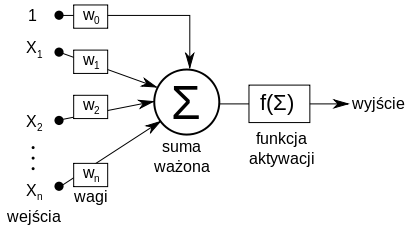
\includegraphics[scale=0.6]{410px-Neuron_McCullocha-Pittsa.png}
\caption{Neuron McCullocha-Pittsa\protect\footnotemark}
\label{fig:neuron}
\end{figure}
\footnotetext{Źródło: \url{https://pl.wikipedia.org/wiki/Plik:Neuron_McCullocha-Pittsa.svg}}

\begin{description}
\item[$X_0, X_1, ..., X_n$] -- \ sygnały wejściowe (przy czym zakładamy, że $X_0=1$),
\item[$W_0, W_1, ..., W_n$] -- \ wagi wzmacniające lub osłabiające rolę sygnału z~wejść,
\item[$f$] -- \ funkcja aktywacji (może mieć różną postać) - w~pierwotnym modelu funkcja typu skoku jednostkowego.
\end{description}

\section{Wielowarstwowe sieci jednokierunkowe}

 W~dalszej części rozważań przyjęto model neuronu podobny do przedstawionego w~poprzednim podrozdziale. Składa się on z~elementu sumacyjnego, do którego dochodzą sygnały wejściowe $x_1, x_2, ..., x_N$ tworzące wektor wejściowy $x=[x_1, x_2, ..., x_N]^T$ pomnożone przez przyporządkowane im wagi $W_{i1}, W_{i2}, ..., W_{iN}$ tworzące wektor wag $i$-tego neuronu $W_i=[W_{i1}, W_{i2}, ..., W_{iN}]^T$ oraz wartość $W_{i0}$ zwana \emph{progiem} (ang. \emph{bias}). Sygnał wyjściowy sumatora oznaczono jako $u_i$:
\begin{equation}
u_i=\sum_{j=1}^{N} W_{ij}x_j+W_{i0}.
\end{equation}
Sygnał ten jest podawany na blok realizujący funkcję aktywacji, skąd trafia na wejście kolejnego neuronu bądź na wyjście sieci \cite{Osowski96}.

Wielowarstwowa sieć neuronowa składa się z~koncepcyjnych warstw. W~podstawowym modelu sieci wszystkie neurony na warstwie są połączone ze wszystkimi neuronami warstwy sąsiedniej. Sygnał dociera do sieci przez \emph{warstwę wejściową} (ang. \emph{input layer}), skąd trafia na wejścia wszystkich neuronów na pierwszej warstwie, gdzie jest przetwarzany przez neuron według powyższego opisu. Następnie trafia na wejścia wszystkich neuronów kolejnej warstwy (jeśli istnieje) i~proces się powtarza, bądź na wyjście sieci. Ostatnia warstwa sieci nazywa się \emph{warstwą wyjściową} (ang. \emph{output layer}). Wszystkie warstwy znajdujące się pomiędzy wejściową a~wyjściową to \emph{warstwy ukryte} (ang \emph{hidden layers}) \cite{Flasinski11}.

\begin{figure}[htp]
\centering
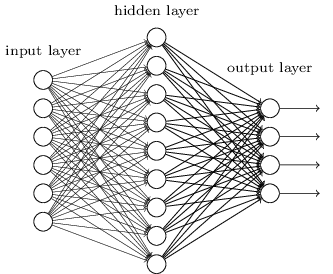
\includegraphics[scale=0.8]{rys/siec_neuronowa.png}
\caption{Przykładowa architektura sieci z~6 wejściami, 9 neuronami na warstwie ukrytej i~4 neuronami na warstwie wyjściowej\protect\footnotemark.}
\end{figure}
\footnotetext{Źródło: \url{http://nb4799.neu.edu/wordpress/?p=246}}

Dobór liczby wejść sieci jest uwarunkowany wymiarem wektora danych $X$. Liczba neuronów na warstwie wyjściowej równa jest rozmiarowi wektora danych zadanych $d$. Problemem pozostaje dobór ilości warstw ukrytych i~ilości neuronów, które się na nich znajdują \cite{Osowski96}.

\section{Uczenie sieci -- wsteczna propagacja błędów}
\label{sec:uczenie_sieci}

Sieć neuronowa pełni rolę układu aproksymującego dane uczące $(x, d)$. W~trakcie uczenia sieci, dobierane są współczynniki tej funkcji aproksymującej -- wektory wag poszczególnych neuronów. Na etapie odtwarzania następuje obliczenie wartości funkcji aproksymującej dla danego wektora wejściowego przy ustalonych wartościach wag \cite{Osowski96}.

Osowski stwierdza, że najlepsze wyniki w~uczeniu sieci można uzyskać poprzez odpowiedni dobór wstępnych wartości wag. Pożądany jest start z~wartości wag zbliżonych do optymalnych. Pozwala to uniknąć utknięcia w~niewłaściwym minimum lokalnym i~jednocześnie przyspiesza proces uczenia. Niestety w~ogólnym przypadku nie istnieje metoda doboru wag będących właściwym punktem startowym dla każdego problemu uczenia się. W~większości zastosowań korzysta się zwykle z~losowego doboru wag, przyjmując rozkład równomierny w~określonym przedziale liczbowym \cite{Osowski96}.

Celem uczenia sieci jest określenie wartości wag neuronów wszystkich warstw sieci w~taki sposób, aby przy zadanym wektorze wejściowym $x$ uzyskać na wyjściu sieci sygnały wyjściowe $y_i$ o~wartościach równych, z~dostateczną dokładnością, wartościom żądanym $d_i$, dla $i=1, 2, ..., M$. Przy założeniu ciągłości funkcji celu najskuteczniejszymi metodami uczenia pozostają gradientowe metody optymalizacyjne \cite{Osowski96}, w~których uaktualnianie wektora wag (uczenie) odbywa się zgodnie ze wzorem:
\begin{equation}
W(k+1)=W(k)+\Delta W,
\end{equation}
 w~którym:
\begin{equation}
\Delta W=\eta p(W),
\end{equation}
$\eta$ jest współczynnikiem uczenia, a~$p(W)$ -- określa kierunek największego spadku wartości funkcji błędu w~przestrzeni wielowymiarowej $W$ \cite{Osowski96}.

Zastosowanie metod gradientowych do uczenia sieci wielowarstwowej wymaga do wyznaczenia kierunku $p(W)$ obliczenia wektora gradientu względem wag wszystkich warstw sieci. Jedynie w~przypadku wag warstwy wyjściowej zadanie to jest określone w~sposób natychmiastowy. Aby określić wspomniany wektor gradnientu dla wektorów pozostałych warstw należy wykorzystać \emph{algorytm propagacji wstecznej} \cite{Osowski96}.

 W~każdym cyklu uczącym wyróżnia się następujące etapy uczenia \cite{Osowski96}:
\begin{enumerate}
\item Analiza sieci neuronowej o~zwykłym kierunku przepływu sygnałów przy założeniu sygnałów wejściowych sieci równych elementom aktualnego wektora $x$. W~wyniku analizy otrzymuje się wartości sygnałów wyjściowych neuronów warstw ukrytych oraz warstwy wyjściowej, a~także odpowiednie pochodne funkcji aktywacji w~poszczególnych warstwach.
\item Realizacja propagacji wstecznej przez odwrócenie kierunków przepływu sygnałów, zastąpienie funkcji aktywacji przez ich pochodne, a~także podanie do byłego wyjścia (obecnie wejścia) sieci wymuszenia w~postaci odpowiedniej różnicy między wartością aktualną i~żądaną. Dla tak utworzonej sieci należy obliczyć wartości odpowiednich różnic wstecznych.
\item Adaptacja wag (uczenie sieci) odbywa się na podstawie wyników uzyskanych w~punktach 1 i~2 dla sieci zwykłej i~sieci o~propagacji wstecznej według odpowiednich wzorów.
\end{enumerate}

Proces opisany w~punktach 1, 2, 3 należy powtórzyć dla wszystkich wzorców uczących, kontynuując go do chwili spełnienia warunku zatrzymania algorytmu. Działanie algorytmu kończy się w~momencie, gdy norma gradnientu spadnie poniżej pewnej wartości $\epsilon$ określającej dokładność procesu uczenia. Dokładniejszy opis metody wstecznej propagacji błędów można znaleźć w~\cite{Flasinski11} oraz \cite{Osowski96}.

Algorytm wstecznej propagacji błędów jest bardzo podobny koncepcyjnie do wcześniej przedstawionego algorytmu Q-learning (patrz wzór \ref{eq:q-learning}). Wykorzystując sieć neuronową jako aproksymator funkcji wartości akcji, w~celu uaktualnienia przybliżenia wartości $Q$ wystarczy nauczyć sieć próbką uczącą $(x,d)$, gdzie $x$ jest reprezentacją pary stan-akcja, a~$d$ nauczoną wartością akcji, ze współczynnikiem uczenia sieci $\eta = \alpha$.

\chapter{Implementacja}
\label{chap:implementacja}

Część implementacyjna pracy została przygotowana głównie w~języku Python 3 wraz z~bibliotekami NumPy i~PyBrain (wykorzystanych w~implementacji algorytmów uczenia się) oraz Pillow i~PyYAML (wykorzystanych w~implementacji interfejsu graficznego gry).

\section{Konwencje stosowane w~implementacji}

Podczas tworzenia implementacji, m.in. ze względu na specyfikę języka Python (np. dynamiczne typowanie), zdecydowano się na zastosowanie pewnych konwencji. W~wypadku ich złamania program nie będzie działał prawidłowo (najprawdopodobniej zakończy działanie z~błędem). Poniżej wymieniono najważniejsze z~nich, wykorzystywane w~strukturach opisywanych w~dalszej części pracy.

Akcja, w~implementacji najczęściej przechowywana pod nazwą \texttt{action} (także \texttt{col}), w~kontekście gry oznacza numer kolumny planszy, licząc kolejno od lewej, rozpoczynając od zera. Na standardowej pustej planszy do Connect 4 można wykonać następujące akcje: 0, 1, 2, 3, 4, 5, 6.

Identyfikator (numer) gracza (\texttt{player\_id}) może przyjmować wartość 1 lub 2, kolejno dla gracza pierwszego (rozpoczynającego grę) i~drugiego.

\section{Plansza oraz stan gry}

Kod odpowiedzialny za logikę gry opisany w~tym podrozdziale znajduje się w~pliku \texttt{gamestate.py} umieszczonym w~folderze \texttt{common} implementacji.

\subsection{Utworzenie planszy oraz wykonywanie ruchów}

Planszę do gry opisuje obiekt \texttt{BoardState}. Nową pustą planszę można utworzyć za pomocą konstruktora tego obiektu, podając jako argumenty wysokość (ilość wierszy) i~szerokość (ilość kolumn) planszy -- dla standardowej gry Connect 4 będzie to 6 wierszy i~7 kolumn. Aby wykonać ruch, należy skorzystać z~metody \texttt{make\_move}, przyjmującej jako argumenty kolejno numer kolumny (od lewej; licząc od zera), w~której gracz umieszcza żeton oraz identyfikator tego gracza.

Metody operujące na obiektach typu \texttt{BoardState}, w~tym \texttt{make\_move}, nie modyfikują stanu obiektu, a~zwracają nowy obiekt zawierający porządane zmiany (obiekty klasy \texttt{BoardState} są więc w~tym sensie \emph{niemutowalne}, niezmienne).

Układ żetonów na planszy jest przechowywany w~obiektach \texttt{BoardState} w~polu \texttt{board}, w~postaci listy kolejnych rzędów od góry do dołu planszy, które z~kolei są listami kolejnych pól od lewej do prawej strony. Pole może mieć wartość \texttt{None} -- być puste lub 1 albo 2, zgodnie z~numerem gracza, który je zajął.

\needspace{5em}

\begin{lstlisting}[language=Python, caption=Operacje na obiektach \texttt{BoardState} -- sesja interaktywna interpretera]
>>> from common.gamestate import BoardState
>>> from pprint import pprint              
>>> board_state = BoardState(6,7)          
>>> pprint(board_state.board)              
[[None, None, None, None, None, None, None],
 [None, None, None, None, None, None, None],
 [None, None, None, None, None, None, None],
 [None, None, None, None, None, None, None],
 [None, None, None, None, None, None, None],
 [None, None, None, None, None, None, None]]
>>> new_board_state = board_state.make_move(3,1)
>>> pprint(new_board_state.board)               
[[None, None, None, None, None, None, None],
 [None, None, None, None, None, None, None],
 [None, None, None, None, None, None, None],
 [None, None, None, None, None, None, None],
 [None, None, None, None, None, None, None],
 [None, None, None, 1, None, None, None]]
>>> pprint(board_state.board)
[[None, None, None, None, None, None, None],
 [None, None, None, None, None, None, None],
 [None, None, None, None, None, None, None],
 [None, None, None, None, None, None, None],
 [None, None, None, None, None, None, None],
 [None, None, None, None, None, None, None]]
>>> new_board_state = new_board_state.make_move(3,2)
>>> pprint(new_board_state.board)
[[None, None, None, None, None, None, None],
 [None, None, None, None, None, None, None],
 [None, None, None, None, None, None, None],
 [None, None, None, None, None, None, None],
 [None, None, None, 2, None, None, None],
 [None, None, None, 1, None, None, None]]

\end{lstlisting}

\subsection{Sprawdzenie rezultatu gry}

\begin{sloppypar}
Funkcję \texttt{game\_result}, umożliwiającą sprawdzenie stanu gry (czy nastąpiła wygrana, remis albo czy rozgrywka wciąż trwa), umieszczono w~definicji obiektu \texttt{BoardState}.
\end{sloppypar}

Metoda ta w~pierszym rzędzie sprawdza, czy na planszy pozostały jeszcze jakieś wolne pola - jeśli nie, zwraca od razu informację o~remisie. Następnie, w~pętli dla każdego z~dwóch graczy, sprawdza, czy jego bierki nie zostały ułożone w~łańcuchu o~długości przynajmniej \texttt{needed\_to\_win}, czyli wymaganej do wygranej (w przypadku klasycznej rozgrywki liczba ta wynosi 4; mechanizm został napisany z~myślą o~możliwej przyszłej modyfikacji). Algorytm polega na próbie wyszukania odpowiednio wielu bierek jednego gracza w~jednej linii kolejno w~poszczególnych wierszach, kolumnach oraz po skosie.

Metoda zwraca słownik (\texttt{dict}) zawierający klucze:
\begin{itemize}
\item \texttt{result} - zawierający ciąg informujący o~rezultacie gry - wygranej (\texttt{'won'}) albo remisie (\texttt{'tied'}),
\item \texttt{player\_id} - zawierający numer gracza (1 lub 2), który wygrał rozgrywkę (obecny tylko wtedy, gdy rezultatem gry jest wygrana któregoś z~graczy)
\end{itemize}

lub \texttt{None}, gdy gra jest jeszcze nierozstrzygnięta.

\subsection{Przekształcenia obiektów klasy \texttt{BoardState}}

\begin{sloppypar}
\begin{description}
\item[\texttt{board\_state.switch\_players()}] -- zwraca obiekt stanu planszy analogiczny do \texttt{board\_state}, z~tym, że żetony pierwszego gracza zostają zamienione z~żetonami drugiego gracza.
\item[\texttt{board\_state.mirror()}] -- zwraca obiekt stanu planszy analogiczny do \texttt{board\_state}, z~tym że pozycje żetonów są odbite symetrycznie względem środkowej kolumny.
\end{description}
\end{sloppypar}

\begin{lstlisting}[language=Python, caption=Przekształcenia obiektów klasy \texttt{BoardState} -- sesja interaktywna interpretera]
>>> pprint(board_state.board)             
[[None, None, None, None, None, None, None],
 [None, None, None, None, None, None, None],
 [None, None, None, None, None, None, None],
 [None, None, None, None, None, None, None],
 [None, None, None, 2, None, None, None],
 [None, None, None, 1, 1, None, None]]
>>> board_state=board_state.make_move(2,2)
>>> pprint(board_state.board)             
[[None, None, None, None, None, None, None],
 [None, None, None, None, None, None, None],
 [None, None, None, None, None, None, None],
 [None, None, None, None, None, None, None],
 [None, None, None, 2, None, None, None],
 [None, None, 2, 1, 1, None, None]]
>>> pprint(board_state.board)             
[[None, None, None, None, None, None, None],
 [None, None, None, None, None, None, None],
 [None, None, None, None, None, None, None],
 [None, None, None, None, None, None, None],
 [None, None, None, 2, None, None, None],
 [None, None, 2, 1, 1, None, None]]
>>> board_state_switched_players=board_state.switch_players()
>>> pprint(board_state_switched_players.board)
[[None, None, None, None, None, None, None],
 [None, None, None, None, None, None, None],
 [None, None, None, None, None, None, None],
 [None, None, None, None, None, None, None],
 [None, None, None, 1, None, None, None],
 [None, None, 1, 2, 2, None, None]]
>>> board_state_mirrored=board_state.mirror()
>>> pprint(board_state_mirrored.board)
[[None, None, None, None, None, None, None],
 [None, None, None, None, None, None, None],
 [None, None, None, None, None, None, None],
 [None, None, None, None, None, None, None],
 [None, None, None, 2, None, None, None],
 [None, None, 1, 1, 2, None, None]]
\end{lstlisting}

\subsection{Stan gry}

Do przechowywania informacji o~aktualnym stanie gry służy obiekt klasy \texttt{GameState}. Kontruktor tego typu przyjmuje kolejno liczbę wierszy (\texttt{rows}) i~kolumn (\texttt{cols}) planszy oraz liczbę żetonów w~linii konieczną do wygranej (\texttt{needed\_to\_win}).

\section{Sterownik gracza}

 W~projekcie przyjęto koncepcję sterownika gracza -- obiektu odpowiadającego za wybór poszczególnych ruchów w~toku gry. Klasa opisująca sterownik gracza musi definiować co najmniej: stałą \texttt{IS\_GUI\_CONTROLLED} oraz dwie metody -- \texttt{configure\_new\_game} i~\texttt{make\_move}.

\needspace{5em}

\lstinputlisting[
    language=Python,
    firstline=6,
    caption=Implementacja sterownika gracza losowego (game\_agents/random.py),
    style=numbers
]{game_agents/random.py}

\section{Agent uczący się ze wzmocnieniem}
\label{sec:impl_agenta}

\begin{sloppypar}
Model agenta uczącego się ze wzmocnieniem został zdefiniowany w~klasie \texttt{ReinforcementPlayer}, znajdującej się w~pliku \texttt{game\_agents/reinforcement\_backend/reinforcementplayer.py}. Jest on wykorzystywany w~sterowniku gracza uczącego się ze wzmocnieniem znajdującym się w~pliku \texttt{game\_agents/reinforcement.py}
\end{sloppypar}

Konstruktor klasy \texttt{ReinforcementPlayer} jako argumenty przyjmuje kolejno obiekt odpowiedzialny za przechowywanie danych (\texttt{data\_storage}) i~konfigurację (\texttt{config}).

Konfiguracja agenta powinna mieć postać słownika o~następującej strukturze:

\needspace{5em}

\lstinputlisting[
    caption=Przykładowa konfiguracja agenta,
    label=lst:konfiguracja-agenta
]{research/reinf_configs/stage_one_best_known_5k.config}

\begin{description}
\item[board] -- opis parametrów planszy, na której agent ma nauczyć się grać: "rows" oznacza liczbę wierszy a~"cols" liczbę kolumn; w~badaniach wykorzystywano standardową planszę z~6 wierszami i~7 kolumnami.
\item[needed\_to\_win] -- liczba bierek w~linii konieczna do wygranej; w~badaniach wykorzystywano standardowe zasady gry.
\item[games\_to\_play] -- ilość gier, które agent ma rozegrać (sam ze sobą) w~ramach nauki.
\item[saving\_rate] -- częstotliwość zapisywania danych (umożliwia kontynuowanie procesu uczenia po jego wcześniejszym przerwaniu).
\item[learining\_rate] -- współczynnik szybkości uczenia się -- $\alpha$, $\eta$.
\item[discount\_factor] -- współczynnik dyskontowania -- $\gamma$.
\item[estimated\_optimal\_future\_value] -- metoda szacowania zdyskontowanej wartości przyszłych akcji $Q_t(s_{t+1}, a_t)$ -- "mean" lub "best\_known" (patrz podrozdział \ref{subsec:agent_implementacja}).
\item[boltzmann\_temperature] -- parametr wykorzystywany w~algorytmie wyboru akcji (patrz podrozdział \ref{sec:boltzmann}).
\item[rewards] -- wartości nagród przyznawanych agentowi w~stanie wygrywającym ("win"), przegrywającym ("loss"), remisu ("tie") lub w~każdym innym ("each\_move").
\end{description}

Pozostałe klucze, jeśli istnieją, mogą być wykorzystywane przez obiekt odpowiedzialny za przechowywanie danych.

\subsection{Implementacja uczenia się ze wzmocnieniem}
\label{subsec:agent_implementacja}

Agent reprezentowany przez obiekt klasy \texttt{ReinforcementPlayer} uczy się grać w~Connect 4 podczas treningu typu "sam ze sobą" -- gra za obu graczy jednocześnie. Grę treningową można uruchomić wywołując metodę \texttt{self\_play\_game} tego obiektu.

\needspace{5em}

\lstinputlisting[
    language=Python,
    firstline=111,
    lastline=121,
    caption=Metoda odpowiedziana za trening agenta,
    style=numbers,
    label=lst:self_play
]{game_agents/reinforcement_backend/reinforcementplayer.py}

Jak pokazano na listingu \ref{lst:self_play}, funkcja najpierw tworzy pustą planszę do gry o~wymiarach zgodnych z~konfiguracją przekazaną wcześniej do konstruktora obiektu. Następnie, aż do zakończenia gry, zmienna \texttt{player\_id} przyjmuje wartość \texttt{1} lub~\texttt{2}. Kolejno następuje wybór akcji zgodnie ze strategią probabilistyczną opartą na~rozkładzie Boltzmanna (patrz podrozdział \ref{sec:boltzmann}) oraz jej wykonanie (poprzez wywołanie metody \texttt{board\_state.make\_move}), uzyskując tym samym od środowiska nowy stan, który jest następnie wykorzystywany do aktualizacji funkcji wartości akcji (wywołanie \texttt{update\_action\_value}). Następnie nowy stan jest zapisywany jako aktualny i~jeśli gra jeszcze się nie skończyła, nadchodzi kolej drugiego gracza, według tego samego schematu.

Warto dokładnie przyjrzeć się wspomnianym metodom.

\lstinputlisting[
    language=Python,
    firstline=71,
    lastline=80,
    caption=Metoda wybierająca akcję na podstawie strategii probabilistycznej,
    style=numbers,
    label=lst:boltzmann
]{game_agents/reinforcement_backend/reinforcementplayer.py}

Metoda z~listingu \ref{lst:boltzmann} pobiera akcje dostępne w~stanie przekazanym jako parametr (numery kolumn, w~których są jeszcze wolne pola), następnie pobiera ich wartości (patrz podrozdział \ref{sec:obiekt_przechowujacy}) przewidywanych zdyskontowanych nagród z~perspektywy gracza \texttt{player\_id} i~wylicza prawdopodobieństwo wyboru każdej z~nich zgodnie z~rozkładem Boltzmanna oraz konfiguracją przekazaną do konstruktora obiektu, a~następnie zwraca wybraną akcję (została wykorzystana metoda z~biblioteki NumPy zaimportowanej pod aliasem \texttt{np}).

\needspace{5em}

\lstinputlisting[
    language=Python,
    firstline=106,
    lastline=110,
    caption=Metoda aktualizująca przybliżenie funkcji wartości akcji,
    style=numbers,
    label=lst:update_action_value
]{game_agents/reinforcement_backend/reinforcementplayer.py}

Metoda przedstawiona na listingu \ref{lst:update_action_value} pobiera odpowiednią wartość wzmocnienia otrzymywanej w~stanie \texttt{state} (na podstawie konfiguracji), następnie wylicza przewidywaną zdyskontowaną sumę przyszłych nagród przy wybraniu akcji \texttt{action} w~stanie \texttt{old\_state} i~przekazuje ją do zapisu (patrz podrozdział \ref{sec:obiekt_przechowujacy}).

\begin{sloppypar}

Warto zauważyć, że w~implementacji zawarto dwa warianty funkcji \texttt{estimated\_optimal\_function\_value} (odpowiednia funkcja jest przypisywana pod ten alias w~konstruktorze obiektu \texttt{ReinforcementPlayer} na podstawie konfiguracji). Obie funkcje przedstawiono na listingu \ref{lst:estimated_optimal_func_val}.

\end{sloppypar}

\needspace{5em}

\lstinputlisting[
    language=Python,
    firstline=81,
    lastline=101,
    caption=Dwa warianty funkcji zwracającej przewidywaną zdyskontowaną sumę nagród,
    style=numbers,
    label=lst:estimated_optimal_func_val
]{game_agents/reinforcement_backend/reinforcementplayer.py}

 W~przypadku, gdy \texttt{state} jest stanem absorbującym, obie funkcje zwracają wartość \texttt{0}.

Pierwsza metoda (\texttt{estimated\_optimal\_future\_value\_mean}) pobiera wszystkie możliwe akcje do wykonania w~stanie \texttt{state} i~"wykonuje je jako przeciwnik" (nie na oficjalnej planszy). Dla wszystkich tak osiągniętych stanów, które nie są terminalami, pobiera wartość najlepszej do wykonania akcji i~zwraca średnią ich wartość.

Druga metoda (\texttt{estimated\_optimal\_future\_value\_best\_known}) działa bardzo podobnie, tyle że nie liczy średniej, a~zwraca wartość najlepszej akcji \texttt{player\_id} po najlepszym ruchu gracza przeciwnego.

Wspomnając o~wyborze najlepszych akcji (ruchów) autor ma na myśli najlepsze względem aktualnego przybliżenia funkcji wartości akcji $Q$.  

\section{Obiekt przechowujący dane}
\label{sec:obiekt_przechowujacy}

 W~poprzednim podrozdziale wspomniano, że agent deleguje przechowywanie danych do zewnętrznego obiektu. Taki obiekt musi posiadać następujące metody:

\begin{description}
\item[\texttt{get\_value\_of\_action(player\_id, state, action)}] -- umożliwiającą pobranie wartości akcji \texttt{action} w~stanie \texttt{state} z~perspektywy gracza \texttt{player\_id},
\item[\texttt{update\_value\_of\_action(player\_id, state, action, learned\_value)}] -- umożliwiającą zmianę wartości akcji \texttt{action} w~stanie \texttt{state} z~perspektywy gracza \texttt{player\_id} na \texttt{learned\_value},
\item[\texttt{save()}] -- zapisującą dane (np. w~pliku na dysku).
\end{description}

 W~niniejszej pracy zaprojektowano klasę \texttt{NeuralStorage}, znajdującą się w~pliku \texttt{storages/neuralstorage.py}. Definiuje ona wspomniane wyżej metody. Obiekt typu \texttt{NeuralStorage} korzysta z~następujących pól konfiguracji agenta:

\begin{description}
\item[board] -- wielkość planszy jest wykorzysywana przy dobieraniu rozmiaru wejścia sieci,
\item[learning\_rate] -- określa szybkość uczenia się sieci neuronowej,
\item[neural\_storage] -- "hidden\_neurons" określa liczbę neuronów na warstwie ukrytej sieci.
\end{description}

\subsection{Implementacja sieci neuronowej}

Do zaimplementowania sieci neuronowej wykorzystano bibliotekę PyBrain. Zastosowano sieć z~\texttt{liczba\_wierszy * liczba\_kolumn + 1} wejściami. Kolejne wejścia oznaczają wartości kolejnych pól na planszy w~danym stanie, od góry do dołu oraz od lewej do prawej strony -- \texttt{0} dla pola pustego, \texttt{1} dla pola zajętego przez pierwszego gracza oraz \texttt{2} oznaczająca pole zajęte przez drugiego gracza. Ostatnie wejście przyjmuje wartość od \texttt{0} do \texttt{liczba\_kolumn-1} i~oznacza numer akcji (kolumny). W~sieci umieszczono jedną warstwę ukrytą o~rozmiarze ustawianym poprzez opcję w~konfiguracji, zawierającą neurony o~sigmoidalnej funkcji aktywacji. Na warstwie wyjściowej znajduje się jeden neuron o~liniowej funkcji aktywacji. Wyjście z~sieci oznacza wartość akcji w~stanie przekazanym na wejściu. Początkowe wagi są losowane z~zakresu $[-1,1]$.

\subsection{Zabiegi ułatwiające uczenie}

Podczas zapisu i~odczytu danych w~sieci neuronowej stosowane są pewne zabiegi, które mają na celu usprawnienie procesu uczenia.

\subsubsection{Odbijanie planszy względem środkowej kolumny}

Jak wspomniano we wstępie, w~Connect 4 występują stany identyczne z~punktu widzenia gry, jednak inaczej reprezentowane na planszy -- są to stany symetryczne względem środkowej kolumny. Skorzystano więc z~tego faktu i~przy każdym zapisie wartości akcji proces uczenia sieci dokonywany jest także dla tej samej wartości dla symetrycznych względem środkowej kolumny stanu i~akcji (nie dzieje się tak, gdy stan zapisywany jest tożsamy ze swoim odbiciem).

\subsubsection{Zapis z~punktu widzenia pierwszego gracza}

Jako że na wejściu sieć nie dostaje informacji, z~punktu widzenia którego gracza ma być obliczona wartość $Q$, przy uczeniu i~odczycie danych z~perspektywy drugiego gracza zastosowano konwencję zamiany wszystkich pól z~wartości \texttt{1} na \texttt{2} i~odwrotnie.

\section{Narzędzia}

Na potrzeby badań przygotowano zbiór skryptów w~językach Python oraz bash.

\subsection{Tworzenie i~uczenie agentów}

Do utworzenia oraz wytrenowania nowego agenta potrzebny jest odpowiedni plik w~formacie JSON\footnote{Oficjalny standard definiujący format JSON można znaleźć pod adresem \url{http://www.ecma-international.org/publications/files/ECMA-ST/ECMA-404.pdf}} (o rozszerzeniu \texttt{.config}) z~opisem zmiennych wykorzystywanych w~procesie uczenia (zawartość pliku powinna być analogiczna do konfiguracji agenta przedstawionej na listingu \ref{lst:konfiguracja-agenta}).

\begin{sloppypar}
Za utworzenie i~wytrenowane agenta na podstawie pliku konfiguracyjnego odpowiada skrypt \texttt{reinforcement\_train.py} (umieszczony w~głównym katalogu implementacji), będący w~istocie "aliasem" do modułu \texttt{game\_agents.reinforcement\_backend.train}.
\end{sloppypar}

Skrypt można uruchomić z~różnymi kombinacjami parametrów. W~najprostszym przypadku skrypt przyjmuje jedynie ścieżkę do pliku konfiguracyjnego, na podstawie którego ma zostać wytrenowany nowy agent. Skrypt wyświetli identyfikator nowoutworzonego agenta (w schemacie nazwa\_konfiguracji-kolejny numer, np. zakładając nazwę pliku konfiguracyjnego test.config nazwą agenta mógłby być ciąg test-1). Proces treningu można przerwać (np. korzystając z~kombinacji klawiszy Ctrl+C) i~wznowić w~późniejszym czasie -- służy do tego opcja \texttt{--resume} (w skrócie \texttt{-r}) z~identyfikatorem treningu (wyświetlonym przez skrypt po uruchomieniu procesu uczenia).

\begin{sloppypar}
Skrypty w~języku bash, automatyzujące trenowanie agentów na poszczególnych etapach badań znajdują się w~folderze \texttt{research/batch\_training\_scripts} pod nazwami \texttt{run\_stage\_X.sh}, gdzie \texttt{X} jest słownym zapisem kolejnych liczb w~języku angielskim oznaczającymi etap badań.
\end{sloppypar}

\subsection{Porównywanie agentów}

 W~celu oceny jakości dobranych wzpółczynników konfiguracji agenta stworzono zestaw narzędzi umożliwiających zestawianie ze sobą agentów w~celu wzajemnej gry.

\begin{sloppypar}
Najprostszym sposobem na zestawienie dwóch agentów w~grze jest skorzystanie ze skryptu \texttt{agents\_duel.py} (umieszczonego w~głównym katalogu implementacji). Opcja \texttt{-{-}list-drivers} (lub krótsza \texttt{-d}) powoduje wypisanie wszystkich dostępnych konfiguracji sterowników gracza (nazwa budowana jest w~postaci \emph{nazwa\_sterownika-nazwa\_konfiguracji-kolejny\_numer\_treningu}). Uruchomienie pojedynku sprowadza się do wywołania skryptu z~trzema parametrami -- kolejno dwoma nazwami sterowników graczy i~liczbą gier, które mają zostać rozegrane. Skrypt zwróci trzy liczby, kolejno: liczbę wygranych pierwszego gracza, liczbę remisów, liczbę wygranych gracza drugiego.
\end{sloppypar}

\begin{lstlisting}[language=bash,caption=Przykładowe wywołanie skryptu \texttt{agents\_duel.py}]
$ agents_duel.py --list-drivers
random
reinforcement-stage_one_best_known_5k-1
reinforcement-stage_one_best_known_5k-2
reinforcement-stage_one_best_known_5k-3
...
$ ./agents_duel.py random random 1000
557 0 443
\end{lstlisting}

Użycie wspomnianego skryptu może być jednak kłopotliwe, gdy występuje potrzeba porównania wielu konfiguracji agentów z~pozostałymi. Z~tego względu postanowiono na podstawie części modułu \texttt{game\_agents.duel}  utworzyć zestaw użytecznych funkcji, umożliwiających przygotowanie w~prosty i~przejrzysty sposób skryptów porównujących wiele konfiguracji agentów. Poniższe funkcje zdefiniowano w~pliku \texttt{research/stage.py}:

\begin{description}
\item[\texttt{run\_duels(pairs, games\_per\_duel)}] -- przyjmuje (uporządkowane) pary (listy lub krotki) nazw sterowników graczy oraz liczbę pojedynków, które mają być przeprowadzone w~każdej z~tych par; wyświetla na ekran ranking konfiguracji na podstawie średniej liczby gier wygranych przez sterowniki przez nie wytrenowanych
\item[\texttt{all\_play\_all(drivers\_names, games\_per\_duel=1)}] -- przyjmuje listę sterowników graczy, a~następnie każdy z~nich dobiera w~parę ze wszystkimi pozostałymi (zarówno jako gracza pierwszego, jak i~drugiego), za wyjątkiem tych wytrenowanych za pomocą tej samej konfiguracji; następnie wywołuje \texttt{run\_duels}
\item[\texttt{all\_with\_random(drivers\_names, games\_per\_duel)}] -- przyjmuje listę sterowników graczy, a~następnie każdy z~nich dobiera w~parę z~graczem losowym (zarówno jako gracza pierwszy, jak i~drugiego); następnie wywołuje \texttt{run\_duels}
\end{description}

\begin{sloppypar}
Warto wspomnieć, że listę wszystkich dostępnych sterowników graczy (agentów wytrenowanych według konfiguracji) można uzyskać wywołując funkcję \texttt{get\_available\_drivers} z~modułu \texttt{game\_agents.duel}.
\end{sloppypar}

\begin{sloppypar}
 Z~wykorzystaniem powyższych funkcji utworzono skrypty rankingujące dla każdego etapu badań. Znajdują się one w~folderze \texttt{research} pod nazwami \texttt{stage\_X\_all\_play\_all.py} i~\texttt{stage\_X\_all\_with\_random.py}, gdzie \texttt{X} jest słownym zapisem kolejnych liczb w~języku angielskim oznaczającymi etap badań.
\end{sloppypar}

\section{Graficzny interfejs gry}

Interfejs graficzny umożliwia w~prosty sposób rozegranie gry w~Connect 4 pomiędzy dwoma osobami, osobą i~agentem komputerowym oraz dwoma agentami. Aby uruchomić aplikację należy skorzystać ze skryptu \texttt{run\_gui.py}. Ze względu na ograniczone miejsce została ona skonfigurowana w~taki sposób, aby w~menu wyboru sterowników graczy pokazywać tylko te sterowniki, które zostały przetestowane za jej pomocą w~części badawczej. Aby zagrać z~innymi sterownikami graczy należałoby zmodyfikować funkcję \texttt{should\_be\_visible} we wspomnianym wcześniej skrypcie.

\begin{figure}[ht]
\centering
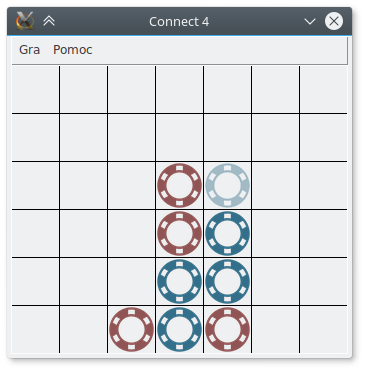
\includegraphics[scale=0.8]{connect4_gui.png}
\caption{Przykładowa rozgrywka w~aplikacji okienkowej}
\label{fig:gui}
\end{figure}

\chapter{Badania}
\label{chap:badania}

Badania polegały na porównywaniu między sobą różnych konfiguracji parametrów uczenia się agenta ze względu na jego skuteczność w~grze z~agentami wytrenowanymi z~użyciem innych konfiguracji oraz z~graczem podejmującym decyzje losowo. Na podstawie każdej wspominanej konfiguracji zostało wytrenowanych pięciu agentów, a~wyniki umieszczone w~tabelach są wynikiem wyciągnięcia średniej z~wyników wszystkich gier rozegranych przez agentów wytrenowanych według danej konfiguracji.

Porównywanie konfiguracji między sobą odbywa się na takiej zasadzie, że każdy agent jest dobierany w~parę ze wszystkimi agentami, którzy nie byli wytrenowani na podstawie jego konfiguracji. Każda para rozgrywa dwie gry -- każdy agent gra raz jako gracz pierwszy i~raz jako gracz drugi. Nie istnieje potrzeba rozgrywania większej liczby gier, gdyż agenci nie wykazują losowości -- odtwarzają jedynie wiedzę, której nauczyli się podczas gier treningowych.

Drugim sposobem porównywania konfiguracji jest zestawianie agentów z~graczem losowym. W~tym wypadku każdy wytrenowany agent rozgrywa grę z~graczem losowym 1000 razy jako gracz pierwszy i~1000 razy jako gracz drugi. Większa liczba rozgrywek jest konieczna ze względu na dużą zmienność wyników gier z~graczem losowym, którą można wyeliminować uśredniając je.

Badania rozpoczęto od następującej, wstępnie dobranej eksperymentalnie konfiguracji, pokazanej na listingu \ref{lst:wstepna_konfiguracja}. Na poszczególnych etapach badań zmieniane są wspominane elementy konfiguracji. W~kolejnych etapach wykorzystywano najlepiej ocenione parametry z~poprzedniego etapu.

Celem eksperymentów jest wyłonienie konfiguracji, według której dałoby się wytrenować agenta mogącego wygrać z~człowiekiem.

\needspace{5em}

\lstinputlisting[
    caption=Wstępna konfiguracja agenta,
    label=lst:wstepna_konfiguracja
]{research/reinf_configs/stage_one_best_known_5k.config}

\section{Etap 1. Metody szacowania wartości przyszłych nagród oraz liczba gier do rozegrania}

 W~pierwszym etapie badań porównano dwie metody wyznaczania szacowanej wartości przyszłych nagród (\texttt{estimated\_optimal\_future\_value}; patrz podrozdział \ref{sec:impl_agenta}) -- \texttt{best\_known} lub \texttt{mean} -- oraz wpływ ilości rozegranych gier treningowych (\texttt{games\_to\_play}) -- 5000, 10.000, 50.000, 100.000 lub 150.000 -- na skuteczność agenta.

\needspace{5em}

\begin{longtable}[c]{|r|c|c|c|}
\caption{\label{tab:results/stage_one_all_play_all}Etap 1. Wzajemne rozgrywki między konfiguracjami} \\
\hline

\multirow{2}{*}{\textbf{Nazwa konfiguracji}} & \multicolumn{3}{|c|}{\textbf{Procent wygranych gier}} \\
\cline{2-4}
&\textbf{średni} & \textbf{max} & \textbf{min} \\
\hline
stage\_one\_best\_known\_50k & 58.44\% & 67.78\% & 52.22\% \\
\hline
stage\_one\_best\_known\_100k & 58.00\% & 64.44\% & 50.00\% \\
\hline
stage\_one\_mean\_150k & 52.00\% & 60.00\% & 43.33\% \\
\hline
stage\_one\_best\_known\_150k & 51.11\% & 57.78\% & 42.22\% \\
\hline
stage\_one\_best\_known\_5k & 50.89\% & 61.11\% & 37.78\% \\
\hline
stage\_one\_mean\_50k & 49.56\% & 58.89\% & 41.11\% \\
\hline
stage\_one\_mean\_5k & 48.00\% & 58.89\% & 35.56\% \\
\hline
stage\_one\_mean\_100k & 46.89\% & 62.22\% & 38.89\% \\
\hline
stage\_one\_mean\_10k & 42.67\% & 48.89\% & 30.00\% \\
\hline
stage\_one\_best\_known\_10k & 39.78\% & 47.78\% & 27.78\% \\
\hline
\end{longtable}


\needspace{5em}

\begin{longtable}[c]{|r|c|c|c|}
\caption{\label{tab:results/stage_one_all_with_random}Etap 1. Rozgrywki z graczem losowym} \\
\hline

\multirow{2}{*}{\textbf{Nazwa konfiguracji}} & \multicolumn{3}{|c|}{\textbf{Procent wygranych gier}} \\
\cline{2-4}
&\textbf{średni} & \textbf{max} & \textbf{min} \\
\hline
stage\_one\_mean\_150k & 79.68\% & 81.60\% & 77.70\% \\
\hline
stage\_one\_mean\_100k & 75.69\% & 78.80\% & 68.65\% \\
\hline
stage\_one\_best\_known\_50k & 71.63\% & 76.45\% & 63.50\% \\
\hline
stage\_one\_best\_known\_100k & 71.12\% & 78.05\% & 62.45\% \\
\hline
stage\_one\_mean\_50k & 70.50\% & 74.80\% & 66.80\% \\
\hline
stage\_one\_best\_known\_10k & 65.66\% & 72.95\% & 59.95\% \\
\hline
stage\_one\_best\_known\_150k & 64.81\% & 74.40\% & 60.65\% \\
\hline
stage\_one\_best\_known\_5k & 62.60\% & 69.35\% & 58.50\% \\
\hline
stage\_one\_mean\_5k & 62.10\% & 68.60\% & 56.00\% \\
\hline
stage\_one\_mean\_10k & 61.16\% & 64.95\% & 57.25\% \\
\hline
\end{longtable}


Przyglądając się danym zaprezentowanym w~tabelach \ref{tab:results/stage_one_all_play_all} oraz \ref{tab:results/stage_one_all_with_random} można zaobserwować pewne zasadnicze różnice -- w~rankingu gier agentów pomiędzy sobą, skuteczniejsza okazała się metoda szacowania funkcji wartości akcji na podstawie najbardziej sprzyjającego przeciwnikowi ruchu i~najbardziej opłacalnej późniejszej akcji agenta. W~rozgrywce z~graczem losowym skuteczniejsza okazała się strategia uśredniająca.

Na tym etapie za najlepszą konfigurację uznano \texttt{stage\_one\_best\_known\_50k}. Przemówiło za tym kilka względów. W~obu zestawieniach ta konfiguracja zajęła wysokie miejsca -- w~tym pierwsze w~grach z~pozostałymi. Czas trenowania rośnie wraz z~liczbą gier do rozegrania, a~metoda wyznaczania przewidywanej wartości akcji metodą uśredniania zajmuje około dwa razy więcej czasu niż poleganie najlepszym znanym ruchu przeciwnika.

\section{Etap 2. Liczba neuronów na warstwie ukrytej sieci}

\begin{sloppypar}
 W~drugim etapie porównano konfiguracje z~różną liczbą neuronów (\texttt{hidden\_neurons}) na warstwie ukrytej sieci, aproksymującej funkcję wartości: 25, 50, 75, 100 lub 125.
\end{sloppypar}

\needspace{5em}

\begin{longtable}[c]{|r|c|c|c|}
\caption{\label{tab:results/stage_two_all_play_all}Etap 2. Wzajemne rozgrywki między konfiguracjami} \\
\hline

\multirow{2}{*}{\textbf{Nazwa konfiguracji}} & \multicolumn{3}{|c|}{\textbf{Procent wygranych gier}} \\
\cline{2-4}
&\textbf{średni} & \textbf{max} & \textbf{min} \\
\hline
stage\_two\_100 & 54.50\% & 65.00\% & 37.50\% \\
\hline
stage\_two\_50 & 53.00\% & 62.50\% & 42.50\% \\
\hline
stage\_two\_75 & 52.00\% & 60.00\% & 45.00\% \\
\hline
stage\_two\_125 & 45.50\% & 67.50\% & 32.50\% \\
\hline
stage\_two\_25 & 43.50\% & 57.50\% & 30.00\% \\
\hline
\end{longtable}


\needspace{5em}

\begin{longtable}[c]{|r|c|c|c|}
\caption{\label{tab:results/stage_two_all_with_random}Etap 2. Rozgrywki z graczem losowym} \\
\hline

\multirow{2}{*}{\textbf{Nazwa konfiguracji}} & \multicolumn{3}{|c|}{\textbf{Procent wygranych gier}} \\
\cline{2-4}
&\textbf{średni} & \textbf{max} & \textbf{min} \\
\hline
stage\_two\_75 & 75.81\% & 79.40\% & 73.65\% \\
\hline
stage\_two\_50 & 75.02\% & 83.80\% & 63.80\% \\
\hline
stage\_two\_25 & 73.75\% & 77.50\% & 70.80\% \\
\hline
stage\_two\_100 & 72.37\% & 83.00\% & 61.00\% \\
\hline
stage\_two\_125 & 66.54\% & 74.75\% & 55.65\% \\
\hline
\end{longtable}


Dobry model powinien być na tyle prosty, by nie być podatny na zbytnie dopasowanie się do danych uczących. Wyraźnie można zaobserwować, że od pewnego momentu im większa liczba neuronów na warstwie ukrytej sieci, tym gorszy wynik. Dlatego zdecydowano się na wybranie konfiguracji \texttt{stage\_two\_50} jako najlepszej w~tym etapie -- utrzymuje stałe drugie miejsce w~obu rankingach oraz używa stosunkowo małej liczby neuronów.

\section{Etap 3. Temperatura w~rozkładzie Boltzmanna}

 W~trzecim etapie porównano różne wartości współczynnika temperatury w~rozkładzie Boltzmanna wykorzystanym do randomizowania wyboru akcji przez agenta w~taki sposób, by zapewnić odpowiednią eksplorację stanów środowiska. Przetestowano wartości \texttt{0.5}, \texttt{1}, \texttt{1.5} oraz \texttt{2}.

\needspace{5em}

\begin{longtable}[c]{|r|c|c|c|}
\caption{\label{tab:results/stage_three_all_play_all}Etap 3. Wzajemne rozgrywki między konfiguracjami} \\
\hline

\multirow{2}{*}{\textbf{Nazwa konfiguracji}} & \multicolumn{3}{|c|}{\textbf{Procent wygranych gier}} \\
\cline{2-4}
&\textbf{średni} & \textbf{max} & \textbf{min} \\
\hline
stage\_three\_1.5 & 56.00\% & 73.33\% & 33.33\% \\
\hline
stage\_three\_1.0 & 51.33\% & 63.33\% & 40.00\% \\
\hline
stage\_three\_2.0 & 48.67\% & 73.33\% & 33.33\% \\
\hline
stage\_three\_0.5 & 42.67\% & 63.33\% & 30.00\% \\
\hline
\end{longtable}


\needspace{5em}

\begin{longtable}[c]{|r|c|c|c|}
\caption{\label{tab:results/stage_three_all_with_random}Etap 3. Rozgrywki z graczem losowym} \\
\hline

\multirow{2}{*}{\textbf{Nazwa konfiguracji}} & \multicolumn{3}{|c|}{\textbf{Procent wygranych gier}} \\
\cline{2-4}
&\textbf{średni} & \textbf{max} & \textbf{min} \\
\hline
stage\_three\_2.0 & 75.04\% & 77.90\% & 70.45\% \\
\hline
stage\_three\_1.5 & 74.50\% & 80.35\% & 70.25\% \\
\hline
stage\_three\_1.0 & 73.60\% & 79.55\% & 59.15\% \\
\hline
stage\_three\_0.5 & 70.38\% & 79.25\% & 61.60\% \\
\hline
\end{longtable}


Obserwując zestawienie jako najlepszą konfigurację wybrano \texttt{stage\_three\_1.5}, która w~pierwszym rankingu uzyskała pierwsze miejsce, a~w drugim drugie, z~bardzo małą różnicą względem pierwszego. Można więc skonkludować, że dość duża losowość wyboru akcji wspomaga proces uczenia, jednak nie powinna ona być zbyt duża. 

\section{Etap 4. Współczynnik dyskontowania}

 W~kolejnym etapie zbadano współczynnik dyskontowania, oznaczający jak ważne są dla agenta przyszłe wzmocnienia. W~konfiguracjach zawarto następujące wartości: \texttt{0} (tylko natychmiastowe nagrody są brane pod uwagę), \texttt{0.25}, \texttt{0.5}, \texttt{0.75} oraz \texttt{1} (liczą się wszystkie szacowane przyszłe wzmocnienia).

\needspace{10em}

\begin{longtable}[c]{|r|c|c|c|}
\caption{\label{tab:results/stage_four_all_play_all}Etap 4. Wzajemne rozgrywki między konfiguracjami} \\
\hline

\multirow{2}{*}{\textbf{Nazwa konfiguracji}} & \multicolumn{3}{|c|}{\textbf{Procent wygranych gier}} \\
\cline{2-4}
&\textbf{średni} & \textbf{max} & \textbf{min} \\
\hline
stage\_four\_1.00 & 58.00\% & 72.50\% & 32.50\% \\
\hline
stage\_four\_0.75 & 54.00\% & 62.50\% & 42.50\% \\
\hline
stage\_four\_0.50 & 52.50\% & 92.50\% & 30.00\% \\
\hline
stage\_four\_0.00 & 48.50\% & 60.00\% & 30.00\% \\
\hline
stage\_four\_0.25 & 36.50\% & 47.50\% & 22.50\% \\
\hline
\end{longtable}


\needspace{5em}

\begin{longtable}[c]{|r|c|c|c|}
\caption{\label{tab:results/stage_four_all_with_random}Etap 4. Rozgrywki z graczem losowym} \\
\hline

\multirow{2}{*}{\textbf{Nazwa konfiguracji}} & \multicolumn{3}{|c|}{\textbf{Procent wygranych gier}} \\
\cline{2-4}
&\textbf{średni} & \textbf{max} & \textbf{min} \\
\hline
stage\_four\_0.00 & 72.41\% & 81.35\% & 65.60\% \\
\hline
stage\_four\_1.00 & 72.35\% & 78.15\% & 68.45\% \\
\hline
stage\_four\_0.50 & 71.77\% & 77.75\% & 64.80\% \\
\hline
stage\_four\_0.75 & 70.28\% & 75.10\% & 63.70\% \\
\hline
stage\_four\_0.25 & 65.38\% & 70.20\% & 62.50\% \\
\hline
\end{longtable}


Do dalszych badań wybrano wartość \texttt{1} współczynnika dyskontowania. W~obu przypadkach konfiguracja z~tą wartością współczynnika zajęła wysokie (odpowiednio pierwsze i~drugie) miejsca.

\section{Etap 5. Współczynnik szybkości uczenia się}

 W~piątym etapie badań zbadano różne wartości współczynnika szybkości uczenia się: \texttt{0.001}, \texttt{0.01}, \texttt{0.05} oraz \texttt{0.1}.

\needspace{5em}

\begin{longtable}[c]{|r|c|c|c|}
\caption{\label{tab:results/stage_five_all_play_all}Etap 5. Wzajemne rozgrywki między konfiguracjami} \\
\hline

\multirow{2}{*}{\textbf{Nazwa konfiguracji}} & \multicolumn{3}{|c|}{\textbf{Procent wygranych gier}} \\
\cline{2-4}
&\textbf{średni} & \textbf{max} & \textbf{min} \\
\hline
stage\_five\_0.05 & 62.00\% & 73.33\% & 46.67\% \\
\hline
stage\_five\_0.1 & 49.33\% & 63.33\% & 43.33\% \\
\hline
stage\_five\_0.001 & 46.00\% & 63.33\% & 26.67\% \\
\hline
stage\_five\_0.01 & 42.00\% & 56.67\% & 36.67\% \\
\hline
\end{longtable}


\needspace{5em}

\begin{longtable}[c]{|r|c|c|c|}
\caption{\label{tab:results/stage_five_all_with_random}Etap 5. Rozgrywki z graczem losowym} \\
\hline

\multirow{2}{*}{\textbf{Nazwa konfiguracji}} & \multicolumn{3}{|c|}{\textbf{Procent wygranych gier}} \\
\cline{2-4}
&\textbf{średni} & \textbf{max} & \textbf{min} \\
\hline
stage\_five\_0.05 & 72.04\% & 81.10\% & 63.45\% \\
\hline
stage\_five\_0.1 & 67.59\% & 77.95\% & 59.05\% \\
\hline
stage\_five\_0.001 & 60.79\% & 63.30\% & 58.00\% \\
\hline
stage\_five\_0.01 & 58.52\% & 68.65\% & 53.05\% \\
\hline
\end{longtable}


 W~przypadku obu zestawień najskuteczniejszy okazał się współczynnik \texttt{0.05}, dlatego też został on wybrany do dalszych etapów badań.

\section{Etap 6. Nagrody}

 W~szóstym etapie badań porównano różne kombinacje wartości nagród. Przygotowano następujące zestawy wzmocnień:

\begin{longtable}[c]{|c|c|c|c|c|}
\caption{\label{tab:results/stage_two_all_play_all}Etap 6. Porównywane zestawy wzmocnień} \\
\hline
\multirow{2}{*}{\textbf{Numer zestawu}} & \multicolumn{4}{|c|}{\textbf{Wartość wzmocnienia}} \\
\cline{2-5}
&\textbf{za wygraną} & \textbf{za przegraną} & \textbf{za remis} & \textbf{za każdy ruch} \\
\hline
1 & 2 & -2 & 0 & -0.01 \\
\hline
2 & 2 & -2 & 0 & 0 \\
\hline
3 & 2 & 0 & 0 & 0 \\
\hline
4 & 0 & -2 & 0 & 0 \\
\hline
5 & 5 & -2 & 0 & 0 \\
\hline
6 & 2 & -5 & 0 & 0 \\
\hline
\end{longtable}

\needspace{5em}

\begin{longtable}[c]{|r|c|c|c|}
\caption{\label{tab:results/stage_six_all_play_all}Etap 6. Wzajemne rozgrywki między konfiguracjami} \\
\hline

\multirow{2}{*}{\textbf{Nazwa konfiguracji}} & \multicolumn{3}{|c|}{\textbf{Procent wygranych gier}} \\
\cline{2-4}
&\textbf{średni} & \textbf{max} & \textbf{min} \\
\hline
stage\_six\_6 & 58.80\% & 76.00\% & 48.00\% \\
\hline
stage\_six\_3 & 53.60\% & 64.00\% & 28.00\% \\
\hline
stage\_six\_2 & 50.40\% & 70.00\% & 34.00\% \\
\hline
stage\_six\_1 & 49.20\% & 58.00\% & 36.00\% \\
\hline
stage\_six\_5 & 45.60\% & 58.00\% & 36.00\% \\
\hline
stage\_six\_4 & 40.80\% & 44.00\% & 36.00\% \\
\hline
\end{longtable}


\needspace{5em}

\begin{longtable}[c]{|r|c|c|c|}
\caption{\label{tab:results/stage_six_all_with_random}Etap 6. Rozgrywki z graczem losowym} \\
\hline

\multirow{2}{*}{\textbf{Nazwa konfiguracji}} & \multicolumn{3}{|c|}{\textbf{Procent wygranych gier}} \\
\cline{2-4}
&\textbf{średni} & \textbf{max} & \textbf{min} \\
\hline
stage\_six\_1 & 75.11\% & 80.85\% & 69.35\% \\
\hline
stage\_six\_2 & 71.81\% & 80.05\% & 59.60\% \\
\hline
stage\_six\_6 & 69.26\% & 75.50\% & 59.15\% \\
\hline
stage\_six\_3 & 66.76\% & 73.30\% & 58.25\% \\
\hline
stage\_six\_4 & 62.74\% & 69.30\% & 59.70\% \\
\hline
stage\_six\_5 & 61.33\% & 66.90\% & 58.40\% \\
\hline
\end{longtable}


Na podstawie wyników porównań możemy stwierdzić, że podobnie nieskuteczni zarówno w~grze z~pozostałymi agentami, jak i~z graczem losowym, byli agenci wytrenowani zgodnie z~konfiguracjami nr 5 oraz nr 6. W~grze z~pozostałymi agentami skuteczni okazali się agenci dużo bardziej karani za porażkę niż nagradzani za wygraną (zestaw 6). W~grze z~graczem losowym przewagę uzyskali agenci, którzy podczas treningu byli nagradzani i~karani w~podobny sposób oraz dodatkowo delikatnie karani za każdy wykonany ruch.

\section{Rozgrywka z~wykorzystaniem interfejsu graficznego}

\begin{sloppypar}
Na zakończenie postanowiono porównać konfiguracje \texttt{stage\_six\_6} oraz \texttt{stage\_six\_1}: najlepsze z~obu rankingów z~poprzedniego porównania, za pomocą gry poprzez interfejs graficzny. Autor rozegrał po jednej grze z~każdym agentem wytrenowanym na podstawie wspomnianych konfiguracji, zarówno jako gracz pierwszy, jak i~drugi, w~rezultacie stwierdzając, że agenci nie są skuteczni w~grze z~człowiekiem. Każda gra skończyła się przegraną agenta.
\end{sloppypar}

\chapter{Podsumowanie}
Pracę rozpoczęto od przedstawienia celu i~struktury pracy, którym podporządkowano dalszą część wywodu. Po zaprezentowaniu zasad gry Connect 4, skupiono się na koncepcji uczenia ze wzmocnieniem. Ukazano jego teoretyczną podstawę -- procesy decyzyjne Markowa, najpopularniejszy algorytm tego typu -- Q-learning oraz techniki mające zapewnić równowagę pomiędzy eksploracją i~eksploatacją środowiska. Następnie dokonano krótkiego wprowadzenia do tematyki sieci neuronowych.

Dla realizacji celu pracy zaprojektowano algorytm bazujący na uczeniu ze wzmocnieniem, umożliwiający uczenie się strategii dla gry Connect4, przy założeniu, że jest ona reprezentowana przez sieć neuronową. Wykonano jego implementację w~języku Python wykorzystując biblioteki do obliczeń numerycznych oraz implementację sieci neuronowej (PyBrain). Opracowano także skrypty umożliwiające tworzenie i~uczenie agentów oraz testowanie jego wyników poprzez rozgrywanie gier pomiędzy agentami lub pomiędzy nimi a~graczem losowym.

Na poszczególnych etapach badań sprawdzano wpływ zmian wartości wybieranych kolejno parametrów uczenia na skuteczność gry agenta. Efekty uczenia się agentów okazały się niesatysfakcjonujące: w~kontekście ich gry pomiędzy sobą najlepsza wśród przeprowadzonych prób konfiguracja osiągnęła średnią wartość 62\% wygranych gier, natomiast najlepsza w~kontekście gry z~graczem losowym -- 79,68\%. W~grze z~człowiekiem agenci popełniali podstawowe błędy (z perspektywy logicznego myślenia).

Uzyskane rezultaty potwierdzają, że uczenie ze wzmocnieniem jest techniką wrażliwą na wartości współczynników. Dla uzyskania lepszej skuteczności konieczne byłyby dalsze badania oraz modyfikacje. Poprawie wyników uczenia mogłaby służyć na przykład modyfikacja reprezentacji stanu przekazywanej na wejście sieci neuronowej aproksymującej funkcję wartości akcji.

%%%%%%%%%%%%
\bibliographystyle{plunsrt}
\bibliography{bibliografia}
\addcontentsline{toc}{chapter}{Bibliografia}

\begin{appendix}
\appendix
\chapter{Instalacja potrzebnego oprogramowania}

Do uruchomienia programów stanowiących część implementacyjną niniejszej pracy konieczny jest interpreter języka Python 3 oraz zainstalowane dodatkowych bibliotek NumPy, SciPy, PyBrain (wykorzystanych w~implementacji algorytmów uczenia się) oraz Pillow i~PyYAML (wykorzystanych w~implementacji interfejsu graficznego gry).

\section{Instalacja interpretera języka Python 3}
\subsection{Linux}
 W~celu instalacji interpretera języka najlepiej skorzystać z~menedżera pakietów, np. apt-get (Debian), pacman (Arch Linux). Pakiet powinien nazywać się, w~zależności od dystrybucji, \texttt{python3} lub \texttt{python}.

\subsection{Windows}
Do instalacji Pythona 3 w~systemie Windows najlepiej wykorzystać gotową dystrybucję wraz z~pakietem bibliotek, np. WinPython\footnote{Oficjalna strona projektu znajduje się pod adresem \url{https://winpython.github.io}}, gdyż instalacja niektórych z~nich (NumPy, SciPy) mogłaby wymagać osobnego doinstalowania narzędzi niezbędnych do ich kompilacji.

\section{Instalacja potrzebnych bibliotek}
\subsection{Linux}
Biblioteki NumPy oraz SciPy najlepiej zainstalować korzystając z~menedżera pakietów, co pozwala na uniknięcie procesu kompilacji oraz instalowania potrzebnych do niego narzędzi. Pakiety powinny nazywać się, podobnie jak w~poprzednim podrozdziale -- w~zależności od dystrybucji, \texttt{\mbox{python3-numpy}} i~\texttt{\mbox{python3-scipy}} albo \texttt{\mbox{python-numpy}} i\,\texttt{\mbox{python-scipy}}.

Pozostałe potrzebne biblioteki można doinstalować np. poleceniem \texttt{pip3} (lub \texttt{pip} -- patrz wcześniejsze uwagi), przechodząc wcześniej w~konsoli do lokalizacji, do której skopiowano pliki dołączone do niniejszej pracy:

\begin{lstlisting}[frame=none, numbers=none]
pip3 install -r requirements.txt
\end{lstlisting}

\subsection{Windows z~WinPython}
Aby uruchomić konsolę systemową wraz z~dostępem do Pythona należy uruchomić program \texttt{WinPython Command Prompt.exe} z~lokalizacji, w~której zainstalowany został WinPython.

Pozostałe potrzebne biblioteki można doinstalować np. poleceniem \texttt{pip}, przechodząc wcześniej w~konsoli do lokalizacji, do której skopiowano pliki dołączone do niniejszej pracy:

\begin{lstlisting}[frame=none, numbers=none]
pip install -r requirements.txt
\end{lstlisting}

\chapter{Opis zawartości płyty CD}

Na płycie dołączonej do pracy znajdują się następujące foldery i~pliki:
\begin{description}
\item[jmlokosiewicz\_inz2016.pdf] -- praca inżynierska w~formacie PDF,
\item[latex] -- folder ze źródłami pracy w~systemie składu \LaTeX,
\item[connect4] -- folder ze źródłami implementacji opisywanej w~rozdziale \ref{chap:implementacja}.
\end{description}

\end{appendix}

\end{document}
